\documentclass{beamer}
\usetheme{metropolis}           % Use metropolis theme
\title{Exploring the role of rewiring on the structure of ecological interaction networks:\newline a simulation-based approach}
\date{July 5, 2024}
\author{Rémi Legrand}
\institute{Laboratoire de Biometrie et Biologie Évolutive}

\begin{document}

\maketitle

\section{Inroduction}

\begin{frame}{\scalebox{.9}{Importance of predicting interactions in a changing environment}}

  \begin{columns}
    \begin{column}{.5\linewidth}
      \includegraphics<1->[width=\linewidth]{figures_slides/ipbes.png}
    \end{column}
    \begin{column}{.6\linewidth}
      \includegraphics<2>[width=\linewidth]{figures_slides/temperature_raising.pdf}
    \end{column}
  \end{columns}
  \vfill
  {\scriptsize \uncover<1->{IPBES report 2019} \hfill \uncover<2->{Hawkins (2020)}}
\end{frame}

\begin{frame}{How to predict interactions}
  \begin{columns}
    \begin{column}{.4\linewidth}
      %\only<3>{Salut}
      %\uncover<3>{Salut}
      \begin{itemize}
      \item<1-> \textbf{Abundances}%
      \item<2-> \textbf{Trait matching} %% The influence of biogeographical and evolutionary
        %% histories on morphological trait-matching and resource specialization
        %% in mutualistic hummingbird--plant networks
      \item<3-> \textbf{Spatio-temporal distribution}%
      \item<4-> \textbf{Others}: adaptation capability: \textbf{rewiring}%
      \end{itemize}
    \end{column}
    \begin{column}{.6\linewidth}
      \includegraphics<1>[width=\linewidth]{figures_slides/abundance.png}%
      \includegraphics<2>[width=\linewidth]{figures_slides/trait_matching.png}%
      \includegraphics<3>[width=\linewidth]{figures_slides/phenology.png}%
      \includegraphics<4>[width=\linewidth]{figures_slides/other_rewiring.png}%
    \end{column}
  \end{columns}
  \vfill
  {\scriptsize \hfill \uncover<4->{Fründ et al (2016)}}
\end{frame}


\begin{frame}{Current method to compute rewiring: Beta dissimilarity}
  \protect\hypertarget{current-method-to-compute-rewiring}{}
  \begin{columns}
    \begin{column}{.5\linewidth}
      \uncover<1->{\textbf{Link dissimilarity: }}
      \uncover<1->{$$\beta_{WN} = \beta_{ST} + \beta_{OS}$$}\\[0.5cm]
      \uncover<3->{\textbf{Downside:}}
      \uncover<3->{%
      \begin{itemize}
        \item Only applicable on binary networks (does not take into account abundances)
      \end{itemize}
      }
    \end{column}
    \begin{column}{.5\linewidth}
      \begin{minipage}{\linewidth}
        \includegraphics<2->[width=\linewidth]{figures_slides/beta_st.png}\\[1cm]
        \includegraphics<2->[width=\linewidth]{figures_slides/beta_os.png}%
      \end{minipage}
    \end{column}
  \end{columns}
  \end{frame}


\begin{frame}{Current method to compute rewiring: Beta dissimilarity}
  \protect\hypertarget{current-method-to-compute-rewiring}{}
  \begin{columns}
    \begin{column}{.5\linewidth}
      \uncover<1->{\scalebox{.9}{\textbf{Individual contribution to rewiring}}}
      \uncover<1->{$$\Delta\beta_{OS,i} = \beta_{OS} - \beta_{OS,\Delta i}$$}\\ [0.5cm]
      \uncover<2->{\textbf{Downsides:}}
      \uncover<2->{
          \begin{itemize}
          \item  $\sum_{i}\beta_{OS,\Delta i} \ne \beta_{OS}$
          \item slow computation
        \end{itemize}}
    \end{column}
    \begin{column}{.5\linewidth}
      \includegraphics<1->[width=\linewidth]{figures_slides/beta_contrib.png}
    \end{column}
  \end{columns}
  \vfill
  {\scriptsize \uncover<1->{Toju et al (2024)}}
  \end{frame}

\section{\scalebox{.8}{Can we better account of abundance for rewiring?}}

\section{Methods}

\begin{frame}{Network notations}
  \centering
  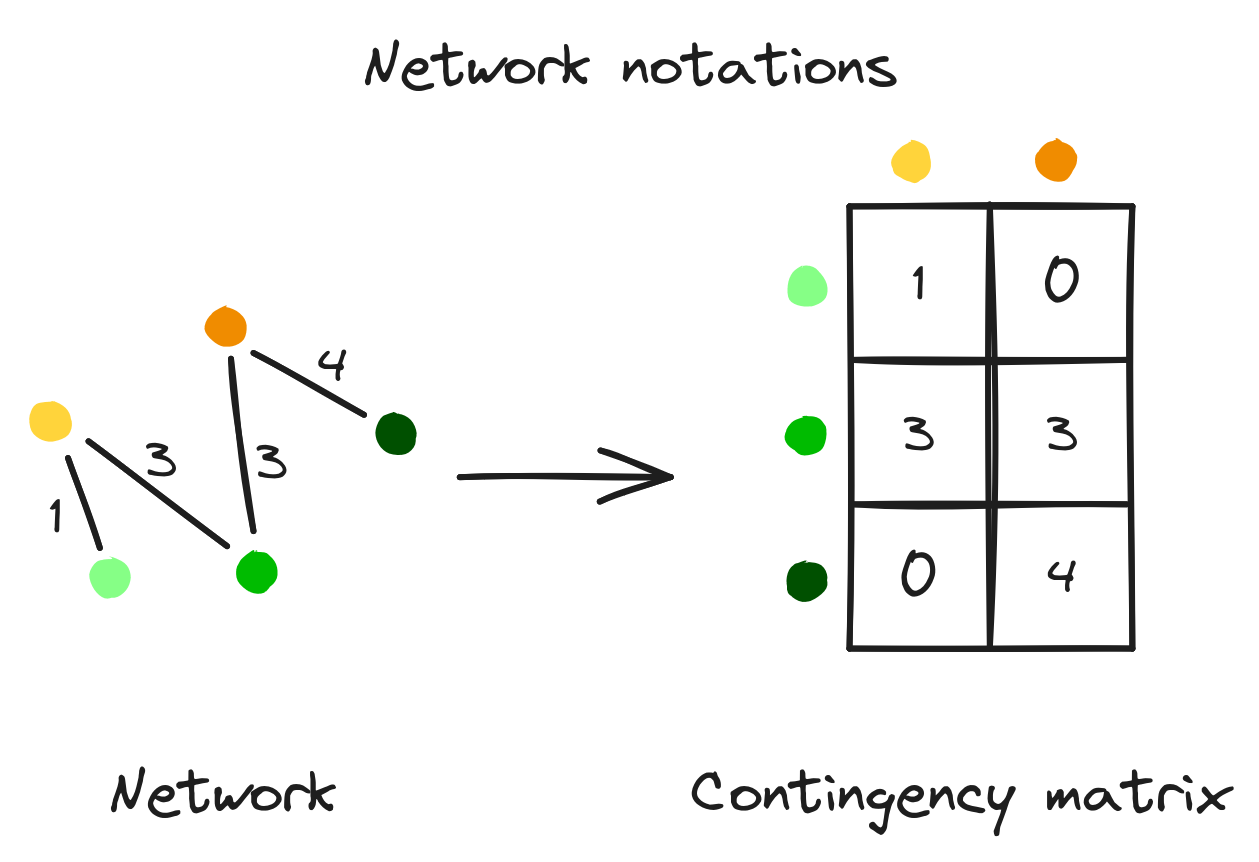
\includegraphics[height=0.7\textheight, keepaspectratio]{figures_slides/netw_notation.png}%
\end{frame}

\begin{frame}{Data simulation process}
  \centering
  \includegraphics<1->[height=0.95\textheight, keepaspectratio]{figures_slides/Netw_generation.png}%
\end{frame}

\begin{frame}{\scalebox{.9}{Estimation of the interaction profile with Correspondance Analysis}}
  \uncover<1->{\textbf{Single network case}}\\ [0.5cm]
  \centering
  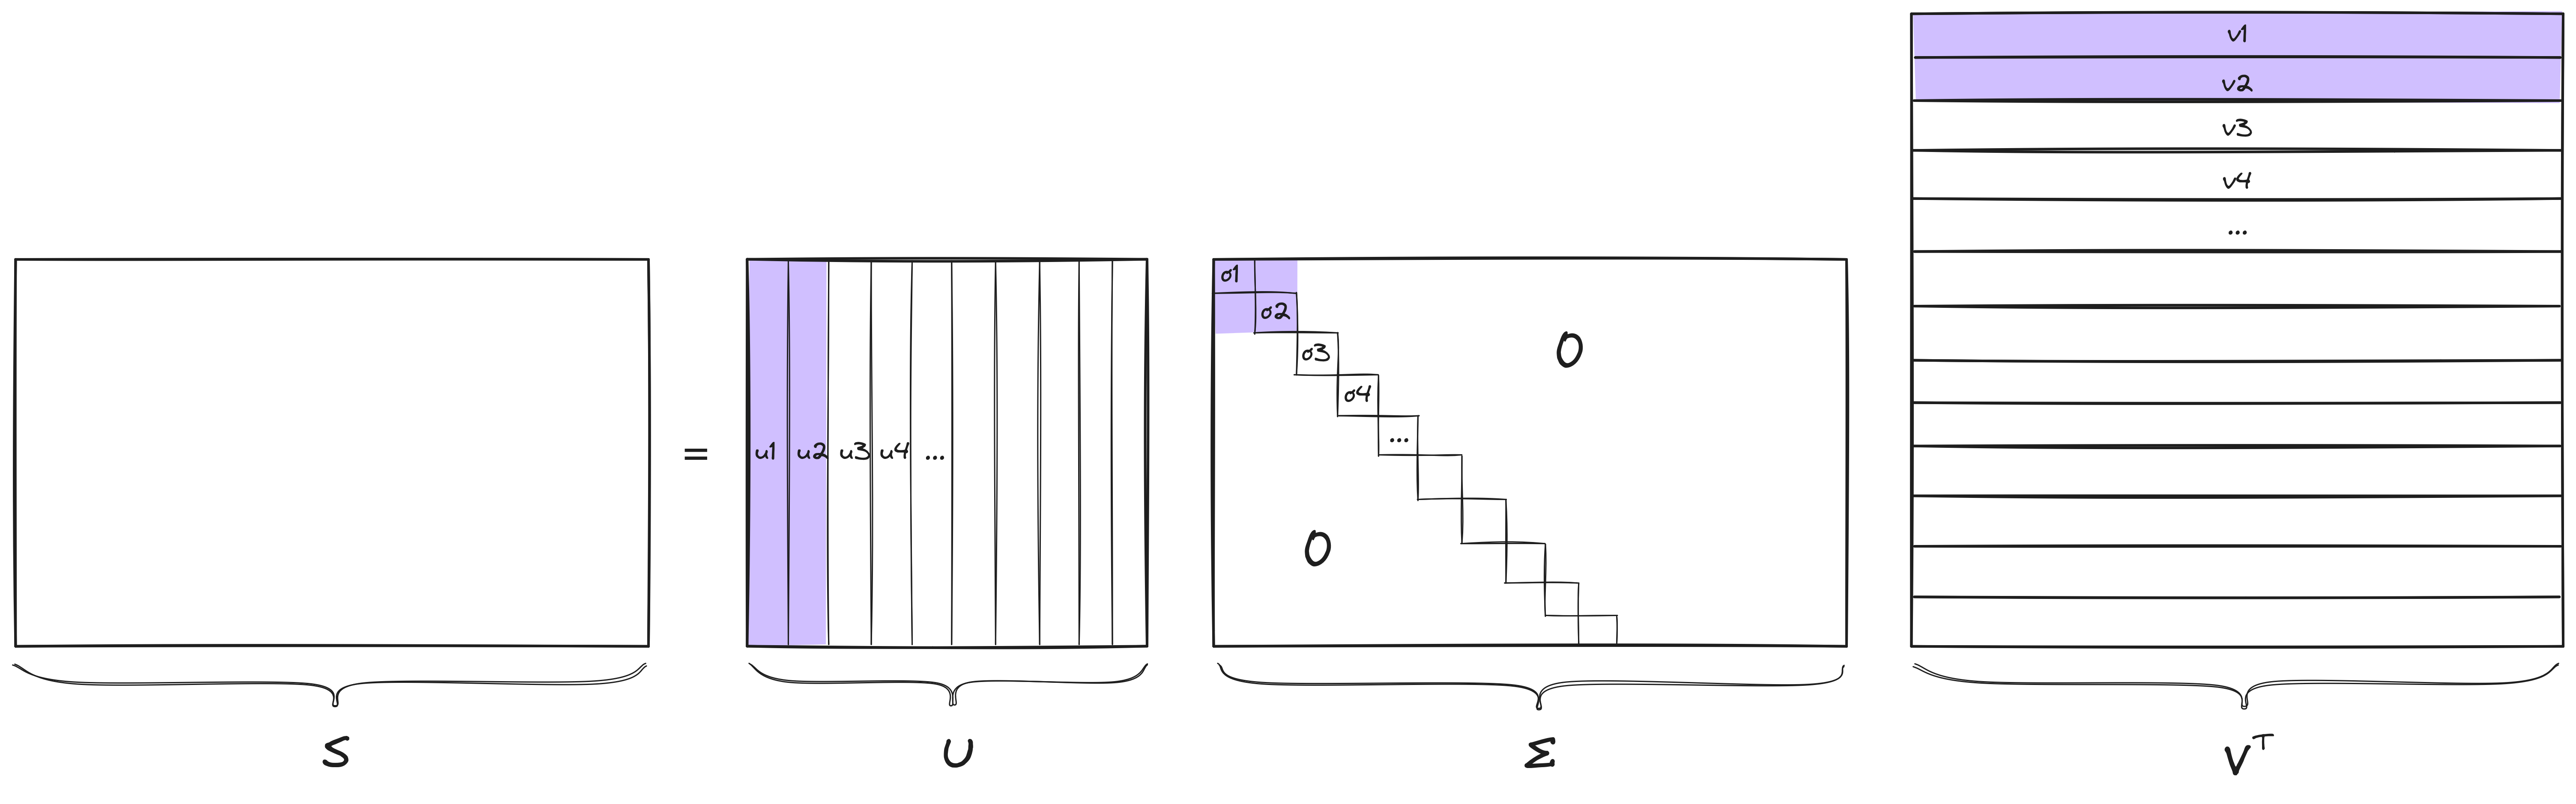
\includegraphics[width=\linewidth, keepaspectratio]{figures_slides/SVD.png}%
\end{frame}


\begin{frame}{\scalebox{.9}{Multiple network extension: Foucart Correspondance Analysis}}
\protect\hypertarget{foucart-ca}{}
\uncover<1->{\textbf{Multiple network case}}\\ [0.5cm]
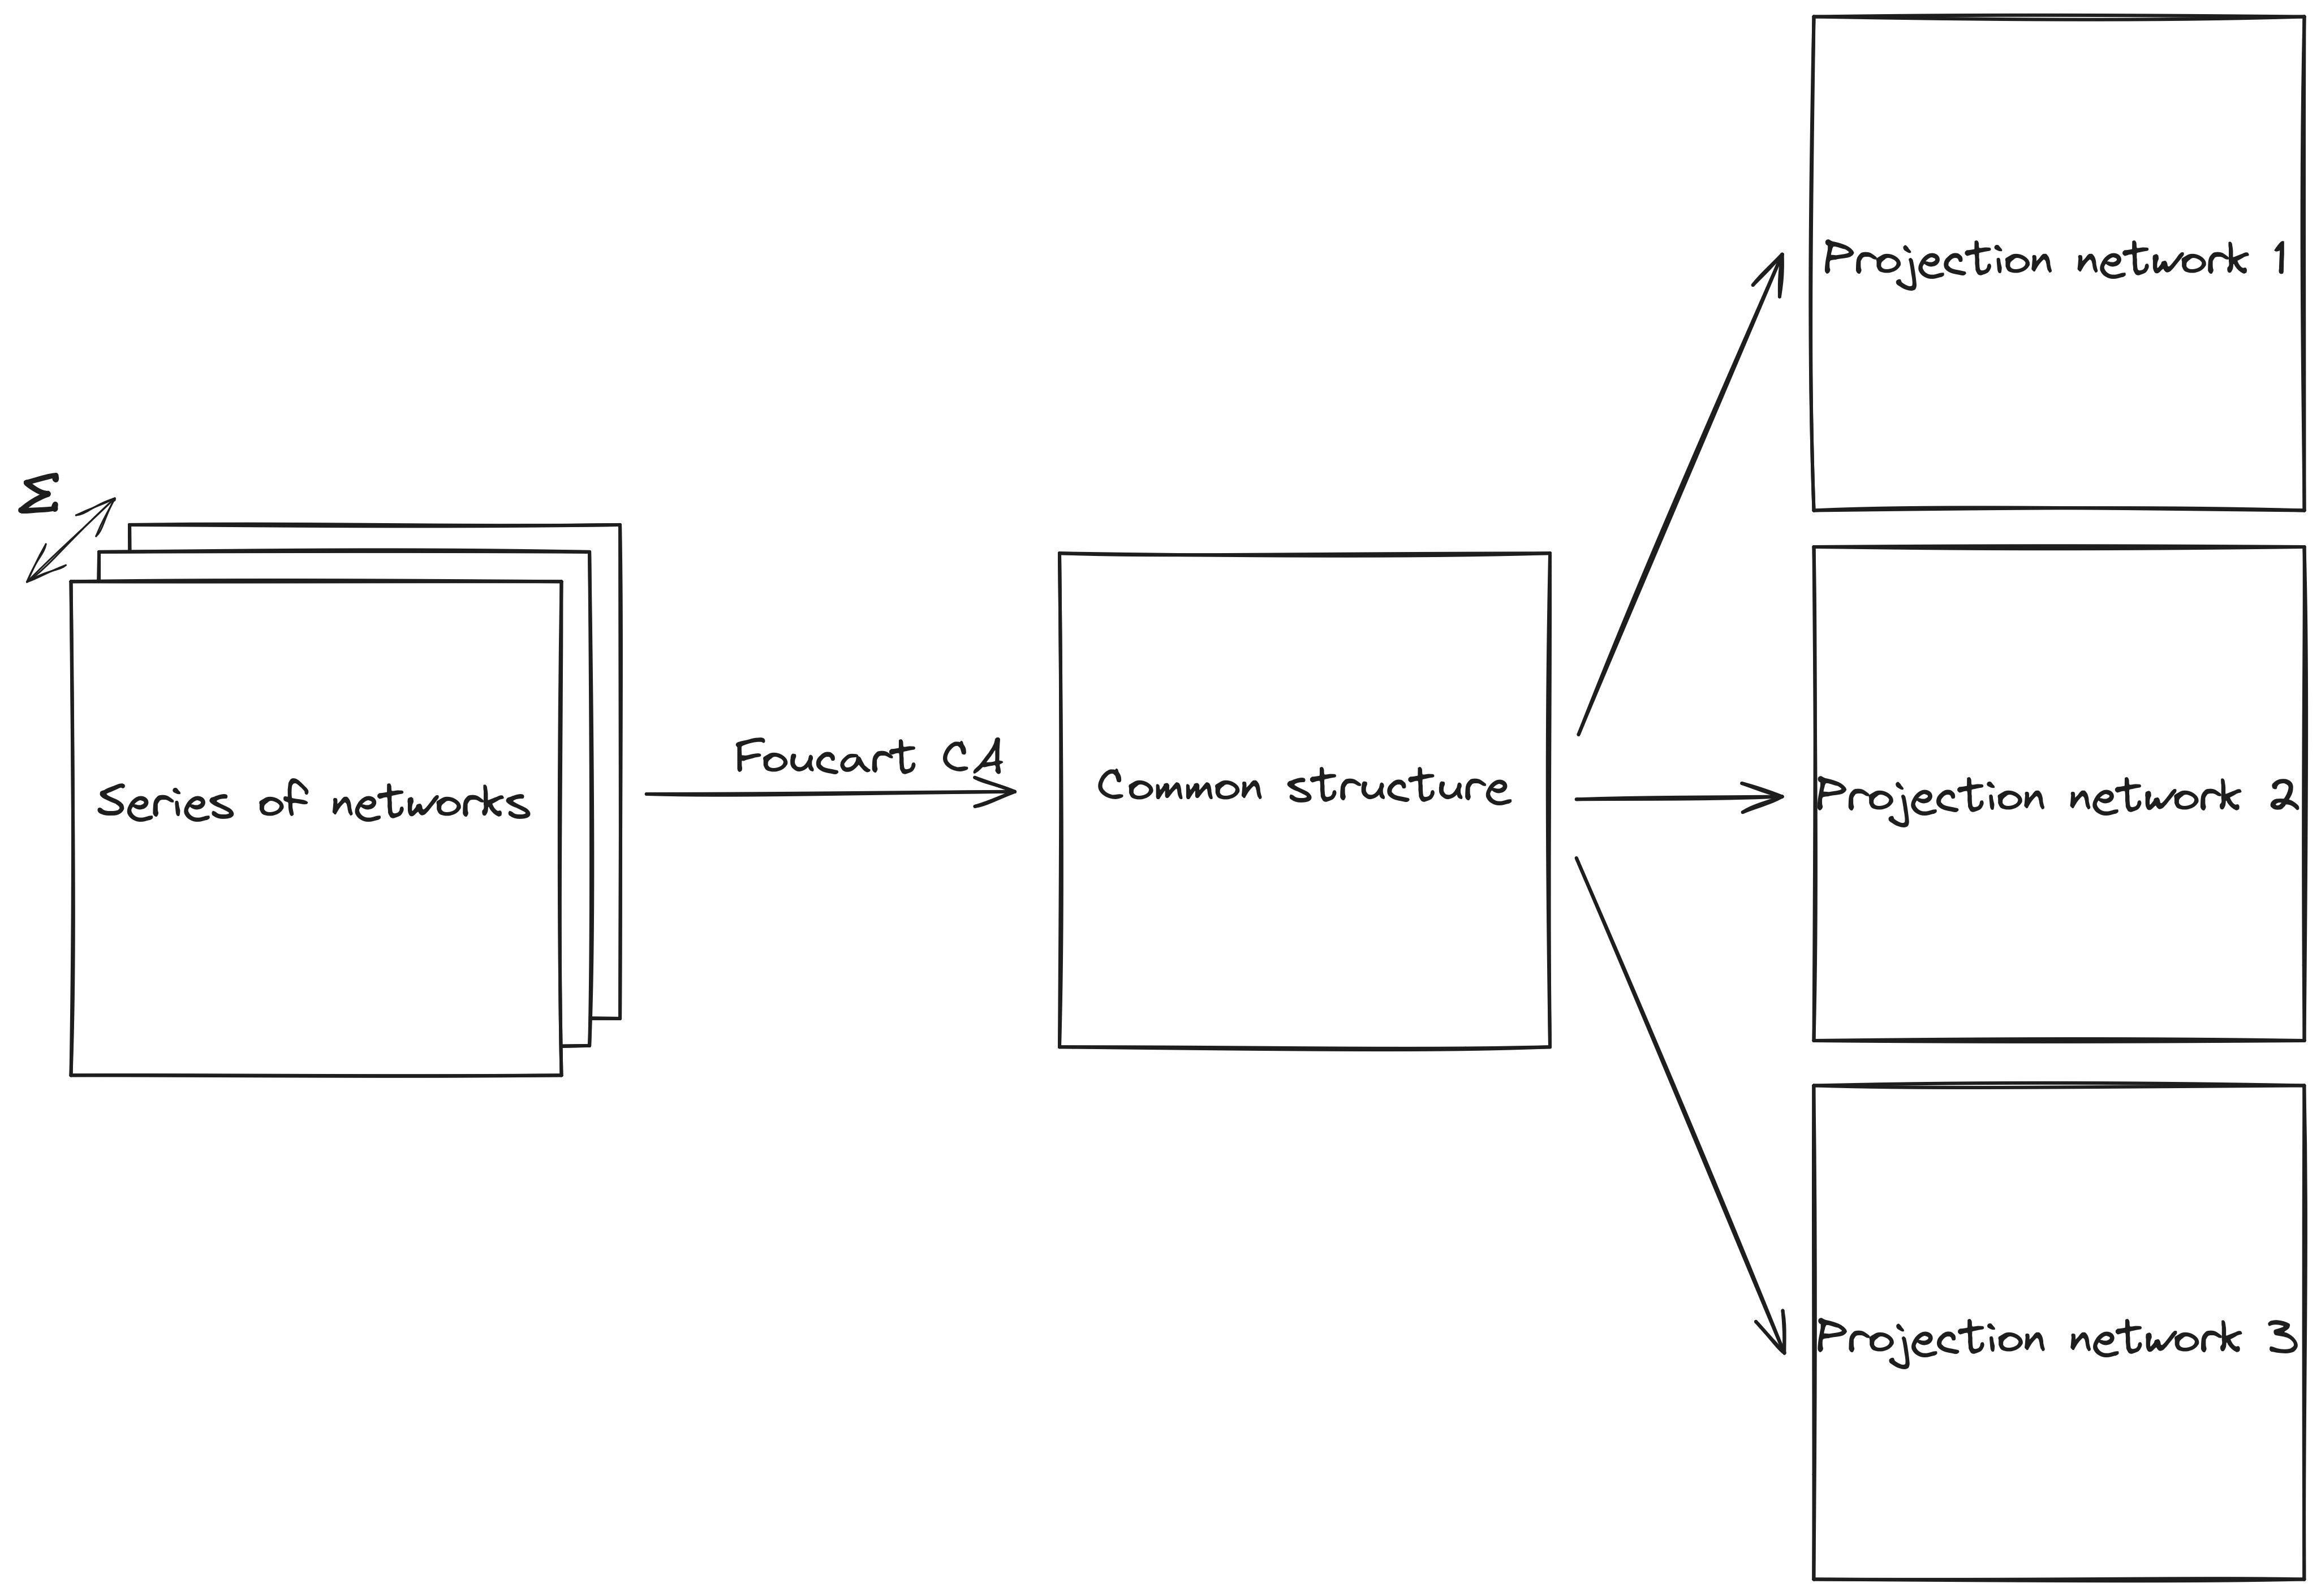
\includegraphics[width=0.9\linewidth]{figures_slides/foucart.png}%
\end{frame}

\section{Results}

\begin{frame}{Compare to beta dissimilarity of co-occuring species}
  \framesubtitle{(or did it?)}
  \includegraphics<1->[width=\linewidth]{figures_slides/rewiring.pdf}%
\end{frame}


\begin{frame}{Why did it not work?}
  \begin{columns}
    \begin{column}{.5\linewidth}
      \includegraphics<1->[width=\linewidth]{figures_slides/foucart_limits.png}%
    \end{column}
    \begin{column}{.5\linewidth}
      \includegraphics<2->[width=\linewidth]{figures_slides/simulation_limits.png}%
    \end{column}
  \end{columns}
\end{frame}

\begin{frame}{Perspectives}
\protect\hypertarget{perspectives}{}
\begin{itemize}
\item
  Take abundances into account in the Beta dissimilarity computation
\item
  Integrate perturbation and the adaptation of species in the simulation
\end{itemize}
\end{frame}

\section*{Thanks for your attention!}


\begin{frame}{Beta dissimilarity}
  \protect\hypertarget{current-method-to-compute-rewiring}{}
  \begin{columns}
    \begin{column}{.5\linewidth}
      \uncover<1->{$$\beta_{dissimilarity} = \frac{|a|+|c|+|b|}{\frac{|a|}{2} + |c|+ \frac{|b|}{2}} - 1$$}
      \uncover<1->{$$\beta_{WN} = \beta_{ST} + \beta_{OS}$$}\vspace{-1em}
      \uncover<1->{$$\Delta\beta_{OS,i} = \beta_{OS} - \beta_{OS,\Delta i}$$}
    \end{column}
    \begin{column}{.5\linewidth}
      \includegraphics<1->[width=\linewidth]{figures_slides/beta_div.png}%
    \end{column}
  \end{columns}
  \end{frame}

\begin{frame}{Trait recovery}
  \includegraphics<1->[width=\linewidth]{figures_slides/supplements/ninter.pdf}%
\end{frame}

\begin{frame}{Trait recovery}
  \includegraphics<1->[width=\linewidth]{figures_slides/supplements/frame_env.pdf}%
\end{frame}

\begin{frame}{Trait recovery}
  \includegraphics<1->[width=\linewidth]{figures_slides/supplements/delta.pdf}%
\end{frame}

\begin{frame}{Trait recovery}
  \includegraphics<1->[width=\linewidth]{figures_slides/supplements/ratio.pdf}%
\end{frame}

\begin{frame}{Trait recovery}
  \includegraphics<1->[width=\linewidth]{figures_slides/supplements/trait.pdf}%
\end{frame}


\end{document}
